\documentclass[tikz]{standalone}
\usepackage{cmap}
\usepackage[T2A]{fontenc}
% \usepackage[utf8x]{inputenc}

\usepackage[russian]{babel}
\usepackage[utf8x]{inputenc}
\usepackage{amsmath}
\usepackage{amssymb}
\usepackage{graphicx}

\usepackage{pgfplotstable}
\usepackage{xcolor}
\definecolor{ochre}{HTML}{e2431e} % #e2431e 0
\definecolor{lightorange}{HTML}{e7711b} % #e7711b 1
\definecolor{lightyellow}{HTML}{f1ca3a} % #f1ca3a 2
\definecolor{lightgreen}{HTML}{6f9654} % #6f9654 3
\definecolor{osci}{HTML}{82FF27}%#82FF27
\definecolor{sky}{HTML}{1c91c0} % #1c91c0 4
\definecolor{violet}{HTML}{43459d} % #43459d 5
% ochre lightorange lightyellow lightgreen osci sky violet 
\usepackage{pgfplots}
\begin{document}
\pgfplotstableset{
	create on use/uz/.style={
	    create col/expr={
	    -\thisrow{e2}/10
	    }
	},
	create on use/du/.style={
	    create col/expr={
	    (0.005*\thisrow{e2}+0.2)/10
	    }
	},
	create on use/di/.style={
	    create col/expr={
	    (0.01*\thisrow{ic}+0.04)
	    }
	},
}
	\begin{tikzpicture}
		    \begin{axis}[
			grid=both,
			scale=1,
			height=5.45cm,
			width=10cm,
			% xmode=log,
			grid style={line width=.0pt, draw=gray!10},
			major grid style={line width=.0pt,draw=gray!50},
			% axis lines=middle,
			% minor tick num=5,
			% xmin=1000, 
			% xmax=11,
			% ymin=0,
			% ymax=5,
			axis on top=true,
			ylabel={$S_x(f)$},
			xlabel={$f$},
			tick style={very thick},
		    % scale=0.5,
		    grid=none,
		    grid style={line width=.0pt, draw=black!20},
		    major grid style={line width=.0pt,draw=black!90},
		    minor y tick num=4,
		    minor x tick num=4,
	    	xmin = 0,
		    ymin = 0,
		    ymax = 15000,
		    xmax = 0.12,
		    % minor x tick num=4,   
			% xmode=log,
			% ymode=log,
		    % xmode=log,ymode=normal,
		    xtick distance=0.02,
		    ytick distance=5000,
		    % ytick distance=0.098171875,
		    % ymax = 1.8,
		    % xmin = 100,
		    % xmax = 1000,
		    % ymin = ,
		    % xmin=-0.1,
		    % ymax = 15,
		    /pgf/number format/.cd,
		    1000 sep={},
		    x tick label style={scale=0.8},
		    y tick label style={scale=0.8},
		    % unit vector ratio*=1 100,
			% yticklabel={
			% \pgfmathparse{\tick/0.098171875/32}
			% \pgfmathifisint{\pgfmathresult}{$\pgfmathprintnumber[int detect]{\pgfmathresult}{}$}%
			% {%
	  %          {$\pgfmathprintnumber[frac, frac denom=32,frac whole=false]{\pgfmathresult}\pi$}
			% }{}
			% },	
			% yticklabel={0}			
			% ytick={1.5707,0.7853,1,2}, 
			% yticklabels={$\frac{\pi}{2}$,%
			% $\frac{\pi}{4}$
			% 1},			
		    % xmax = 40,
		    % ticklabel style={font=\tiny,fill=white},    
		    % axis lines=middle, 	
		    % xlabel style={right, xshift=1em},
		    % ylabel style={above},	
		    x label style={at={(axis description cs:0.5,-0.02)},anchor=center},
		    y label style={at={(axis description cs:0.05,0.5)}}	,
		     % y dir=reverse
		     % restrict y to domain=0:2,    		
		     % restrict x to domain=0:3000,    		
			% legend style={
			% at={(rel axis cs:0,1)},
			% anchor=north west,draw=none,inner sep=0pt,fill=gray!10}
		legend style={
			% cells={anchor=east},
			legend pos=north west,
		},
  x tick label style={
        /pgf/number format/.cd,
            fixed,
            % fixed zerofill,
            precision=2,
        /tikz/.cd
    }
		]
	     % \xdef\C{5e-8}
	     % \xdef\R{13000}
	      % \addplot+[scatter,only marks,
             % domain=0:8,samples=100]
            % {exp(x)};
		\node[above right,inner sep=-0.5pt] (russell) at (rel axis cs:0,0)
    {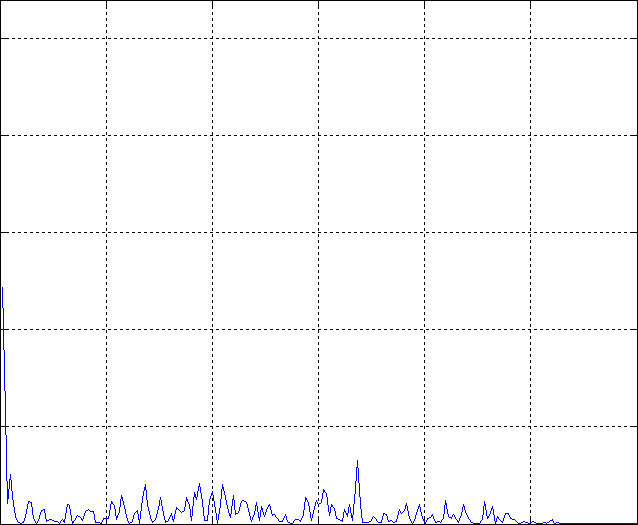
\includegraphics[trim={0 0 0 8.2cm},clip,width=8.48cm]{out/51_n32.png}};
		% \addplot +[mark=*, line width=1pt, mark size=1.2pt, solid,draw=lightorange] plot [error bars/.cd, y dir = both, y explicit,x dir = both, x explicit] table [ x=f_Hz, y=U_mV] {../data/steel.tsv};
		% \addlegendentry{$U_c=10$ В}
		% \addplot +[mark=*, line width=0.4pt, mark size=0.4pt, solid,violet] plot [error bars/.cd, y dir = both, y explicit,x dir = both, x explicit] table [ x=uz, y=ic, y error=di, x error=du] {../data/ex2.tsv};
		% \addlegendentry{$U_c=2\hphantom{0}$ В}

		% \addplot +[mark=*, line width=0.4pt, mark size=0.4pt, solid,ochre] plot [error bars/.cd, y dir = both, y explicit,x dir = both, x explicit] table [ x=uz, y=ic, y error=di, x error=du] {../data/ex1.tsv};
		% \addlegendentry{$U_c=0.5$ В}
		% \addplot +[mark=square*, line width=1.2pt, mark size=3pt, solid,red] plot [error bars/.cd, y dir = both, y explicit] table [ x=ip, y=id, ] {../data/5a2.tsv};\addlegendentry{$U_\text{рез}=120$ В}
		% \addplot +[mark=triangle*, line width=1.2pt, mark size=3pt, solid,magenta] plot [error bars/.cd, y dir = both, y explicit] table [ x=ip, y=id, ] {../data/5a3.tsv};\addlegendentry{$U_\text{рез}=\hphantom{1}90$ В}
		% \addplot[color=red,samples=10, domain=-2:0]{2.54*(x+1.7)}; 10v
		% \addplot[color=blue,samples=10, domain=-2:0]{8.52*(x+1.33)}; 2v
		% \addplot[color=ochre,samples=10, domain=-2:0]{10.36*(x+1.26)}; 0.5v
		    \end{axis}

		\end{tikzpicture}	
\end{document}